%%
%% Beginning of file 'sample.tex'
%%
%% Modified 2005 December 5
%%
%% This is a sample manuscript marked up using the
%% AASTeX v5.x LaTeX 2e macros.

%% The first piece of markup in an AASTeX v5.x document
%% is the \documentclass command. LaTeX will ignore
%% any data that comes before this command.

%% The command below calls the preprint style
%% which will produce a one-column, single-spaced document.
%% Examples of commands for other substyles follow. Use
%% whichever is most appropriate for your purposes.
%%
%%\documentclass[12pt,preprint]{aastex}

%% manuscript produces a one-column, double-spaced document:

%\documentclass{article}
%\documentclass[twocolumn]{aastex6}
\documentclass{aastex6}
%\documentclass[iop]{emulateapj}

%% preprint2 produces a double-column, single-spaced document:
%\documentclass[preprint2]{aastex}

%% Sometimes a paper's abstract is too long to fit on the
%% title page in preprint2 mode. When that is the case,
%% use the longabstract style option.

%% \documentclass[preprint2,longabstract]{aastex}

%% If you want to create your own macros, you can do so
%% using \newcommand. Your macros should appear before
%% the \begin{document} command.
%%
%% If you are submitting to a journal that translates manuscripts
%% into SGML, you need to follow certain guidelines when preparing
%% your macros. See the AASTeX v5.x Author Guide
%% for information.

%Packages
%\usepackage[colorlinks=true,linkcolor=blue,citecolor=blue]{hyperref}
\usepackage{graphicx}
\usepackage{float}
%\usepackage{caption}
%\usepackage{subcaption}
\usepackage[caption=false]{subfig}

\usepackage{natbib}
%\usepackage{pdflscape}
\bibliographystyle{astroads}

\newcommand{\vdag}{(v)^\dagger}
\newcommand{\DHSres}{299 - 334}
\newcommand{\DHSresApprox}{300}
\newcommand{\DHSgap}{0.04}
\newcommand{\degree}{^\circ}
\newcommand{\SOSSrange}{0.6 - 2.5~$\mu$m}
\newcommand{\SOSSrangeto}{0.6 to 2.5~$\mu$m}

%% You can insert a short comment on the title page using the command below.

%\slugcomment{DHS White Paper}

%% If you wish, you may supply running head information, although
%% this information may be modified by the editorial offices.
%% The left head contains a list of authors,
%% usually a maximum of three (otherwise use et al.).  The right
%% head is a modified title of up to roughly 44 characters.
%% Running heads will not print in the manuscript style.

\shorttitle{NIRCam Flux Calibration}
\shortauthors{Schlawin et al.}

%% This is the end of the preamble.  Indicate the beginning of the
%% paper itself with \begin{document}.

\begin{document}

%% LaTeX will automatically break titles if they run longer than
%% one line. However, you may use \\ to force a line break if
%% you desire.

\title{NIRCam Faint and Bright Flux Calibration Plan}

%% Use \author, \affil, and the \and command to format
%% author and affiliation information.
%% Note that \email has replaced the old \authoremail command
%% from AASTeX v4.0. You can use \email to mark an email address
%% anywhere in the paper, not just in the front matter.
%% As in the title, use \\ to force line breaks.

\author{E. Schlawin, Jarron Leisenring, M. Rieke, G. Rieke, K. Misselt}
\affil{Steward Observatory, Tucson AZ 85721}
\email{eas342@email.arizona.edu}

%% Notice that each of these authors has alternate affiliations, which
%% are identified by the \altaffilmark after each name.  Specify alternate
%% affiliation information with \altaffiltext, with one command per each
%% affiliation.

\altaffiltext{1}{Hubble Postdoctoral Fellow}

%% Mark off your abstract in the ``abstract'' environment. In the manuscript
%% style, abstract will output a Received/Accepted line after the
%% title and affiliation information. No date will appear since the author
%% does not have this information. The dates will be filled in by the
%% editorial office after submission.

\begin{abstract}
The James Webb Space Telescope (JWST) offers unprecedented sensitivity and stability for science.
Several of the science areas, such as supernovae photometry for dark energy measurements will require high accuracy absolute calibration.
We discuss a program to identify calibrators at the low end of the flux scale that will not saturate the NIRCam full frame mode.
We obtain ground based photometry and spectroscopy of three clusters to find solar analog G2 V stars and a solar model spectrum to infer the fluxes in the NIRCam bands.
Additionally, we discuss some of the NIRCam modes that can be used to tie JWST calibrations directly to bright stars which have been calibrated against emissive reference spheres with the Midcourse Space Experiment (MSX).
\end{abstract}

%% Keywords should appear after the \end{abstract} command. The uncommented
%% example has been keyed in ApJ style. See the instructions to authors
%% for the journal to which you are submitting your paper to determine
%% what keyword punctuation is appropriate.

\keywords{instrumentation: spectrographs}

%% From the front matter, we move on to the body of the paper.
%% In the first two sections, notice the use of the natbib \citep
%% and \citet commands to identify citations.  The citations are
%% tied to the reference list via symbolic KEYs. The KEY corresponds
%% to the KEY in the \bibitem in the reference list below. We have
%% chosen the first three characters of the first author's name plus
%% the last two numeral of the year of publication as our KEY for
%% each reference.


%% Authors who wish to have the most important objects in their paper
%% linked in the electronic edition to a data center may do so by tagging
%% their objects with \objectname{} or \object{}.  Each macro takes the
%% object name as its required argument. The optional, square-bracket 
%% argument should be used in cases where the data center identification
%% differs from what is to be printed in the paper.  The text appearing 
%% in curly braces is what will appear in print in the published paper. 
%% If the object name is recognized by the data centers, it will be linked
%% in the electronic edition to the object data available at the data centers  
%%
%% Note that for sources with brackets in their names, e.g. [WEG2004] 14h-090,
%% the brackets must be escaped with backslashes when used in the first
%% square-bracket argument, for instance, \object[\[WEG2004\] 14h-090]{90}).
%%  Otherwise, LaTeX will issue an error. 

\section{Introduction}

The James Webb Space Telescope \citep[JWST; e.g.][]{gardner2006SSRv} will need absolute calibration to accomplish its science goals.
One are where accurate flux calibration is especially important is dark energy science, which makes use of type Ia supernovae as standard candles.
Absolute fluxes are especially important for improving type Ia supernova luminosity distances and thus the expansion history of the Universe.
JWST will have no standard calibration sources onboard so all calibration must be performed with astronomical sources.\footnote{While NIRCam had internal lamps in original designs, the envelopes for the filaments broke during testing so the sources were removed.}

The JWST flux calibration effort has been described in \citet{gordon2009fluxplan1} and \citet{gordon2011fluxplan2}.
It is still being developed and refined.
Figure \ref{fig:JWStcalsWideF} shows several of the sources that will likely be used for flux calibration.
These include three categories: 1) hot stars (white dwarf and OB stars) 2) G-stars (which are solar-like) and 3) A-type stars.
The variety of spectra used in JWST calibration can mitigate against biases when models are used to convert flux in one filter to the expected flux in another filter.

The original flux calibration effort has mainly bright stars ($K \lesssim 15$).
Example spectra for these calibrators are shown in Figure \ref{fig:JWStcalsWideF} with saturation and sensitivity limits of NIRCam's wide filters.
Many of these spectra will saturate the NIRCam detectors when used in full frame (shown as the middle parts of the black ``error bars'').
Furthermore, there may be systematic errors when observing faint targets and low detector well depths.
\textcolor{red}{[Have a detector person - Karl, Jarron or George read the rest of this paragraph:]}
As an example of a systematic detector effect, consider charge traps within a detector.
These traps would tend to decrease the measured number of electrons per second on the first exposure because they would trap electrons  that would not be read out by an amplifier.
For bright sources, the effect of the traps would be smaller since they would quickly be a small fraction of the flux.
For faint sources, however, the traps would be a larger fraction of the incoming electrons.

\begin{figure}[!hbtp]
\centering
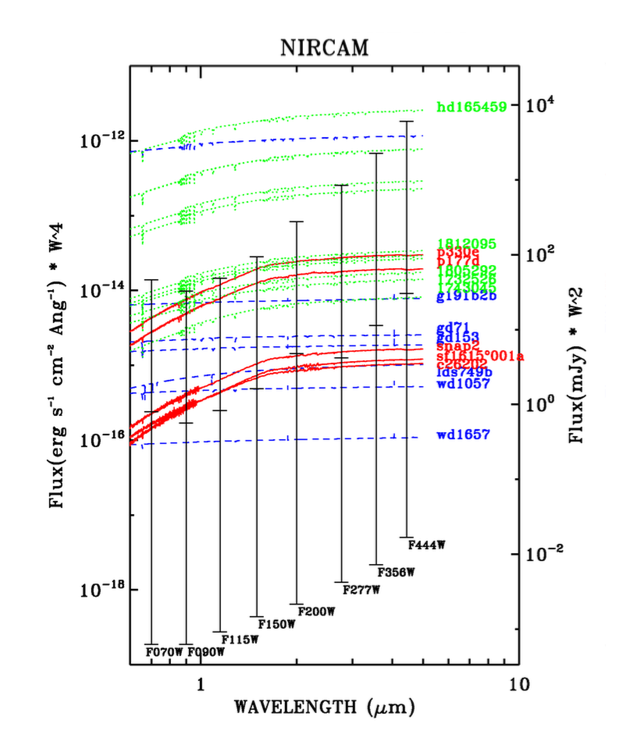
\includegraphics[width=.6\columnwidth]{nircam_wide_filters.png}
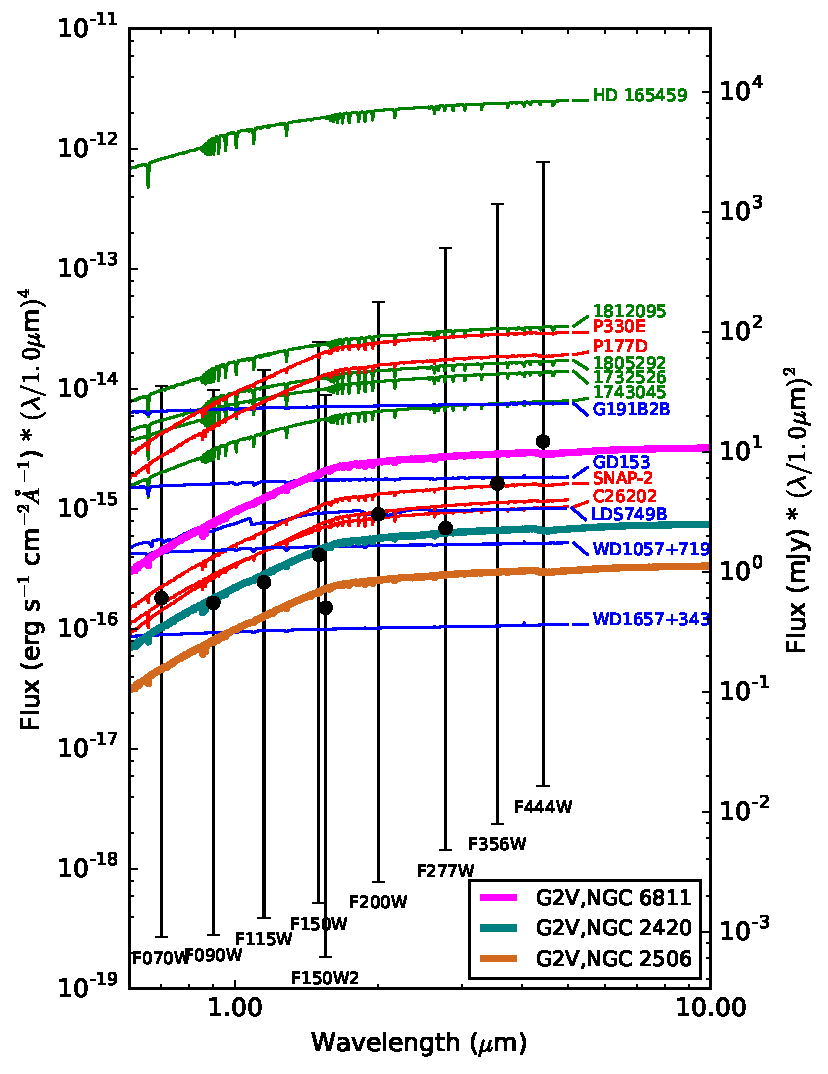
\includegraphics[width=.3\columnwidth]{calspec_and_new_clust.pdf}
\caption{{\it Left:} The NIRCam subarray saturation, full frame saturation and 10~$\sigma$ sensitivity limits for wide band imaging from \citet{gordon2011fluxplan2}. The three values are shown as upper, middle and lower limit error bars respectively. For comparison, three classes of JWST calibrators are shown: hot stars including white dwarfs (blue), A-type stars (green) and G-type stars (red).
Additional faint calibrators are needed to extend the sample from \citet{gordon2011fluxplan2} towards the faint limits of NIRCam.
{\it Right:} The new expected G2 V calibrators as compared to the faintest G-type star in the calibration plan.}\label{fig:JWStcalsWideF}
\end{figure}

In this report, we discuss a NIRCam-led effort to identify and calibrate stars to add to the JWST sample on the fainter end around $K \approx 15$.
We choose the method of \citet{rieke2008absIRcal}, which uses solar-like stars for flux calibration.
The basic rationale is that the Solar spectrum is well measured across JWST's wavelengths \citep[0.6~$\mu$m to 29~$\mu$m][]{gardner2006SSRv} and has highly accurate models for its spectrum.
When solar-like stars are identified, one can use these models to convert from one photometric or spectroscopic band to another.
We identify solar-like stars in open clusters because it allows us to average over multiple stars and to cross-calibrate with bright references within the cluster.
The color magnitude diagram of the cluster also allows us to identify solar like stars and aids in the corrections for extinction.

\section{Cluster Properties}

Our team examined open clusters from the WEBDA database\footnote{https://www.univie.ac.at/webda/webda.html} to find clusters most suitable for flux calibration with solar-like stars.
The parameters under consideration were the the following:
\begin{itemize}
\item {\bf Age:} For the methods to work, the solar-mass stars must be on the main sequence. If we require that a solar mass star have $T_{\rm eff}$ = 5780 +/- 100 K, the cluster would have to be between 0.3 Gyr and 10 Gyr using Dartmouth evolutionary models \citep{dotter2008dartmouth}. Furthermore, the age should be $\lesssim$7 Gyr to avoid main sequence turnoff of near-solar stars.
\item {\bf Extinction} Extinction should be as small as possible to minimize the effects of extinction correction to photometry. Of the clusters found, E(B-V) $\lesssim 0.1$.
\item {\bf Distance Modulus} The cluster must be distant enough to not saturate NIRCam's wide filters in full frame mode. The most easily saturated filter for G stars is the F090W, which corresponds to a G2~V star of 15.9 in the $K$ band. This means the true distance modulus $(m - M)_0$ should be 12.6 for a solar absolute K=3.28 \citep{binney1998book}.
The longer wavelength wide band filters (F200W, F277W, F356W, and F444W) will not saturate for a true distance modulus larger than 11.8.
If one assumes an extinction of E(B-V) = 0.05 and a Galactic average extinction law \citep{cardelli1989}, the visual distance modulus $(m- M)_V$ should be an additional 0.14 mag.
Thus, to calibrate all filters, the visual distance modulus $(m- M)_V$ should be larger than 11.94.
\item {\bf Metallicity} Ideally, the cluster should have near-solar metallicity so that the solar mass stars have a luminosity near 1 $L_\sun$ and a G2~V type spectrum.
\item {\bf Compactness} The cluster should be relatively compact compared to NIRCam's FOV (2'$\times$2' per module). We selected clusters $\lesssim 15\arcmin$
\item {\bf Ancillary data} The clusters should have ancillary photometry from multiple observatories for cross-calibration. We preferred clusters with 2MASS, WISE and IRAC measurements.
\item {\bf Visibility} The clusters should be spread out in ecliptic longitude to ensure that at least one is visible during the commissioning period.
\end{itemize}

With all these considerations in play, we selected NGC 2420 as the best fit for the multiple criteria.
The only parameter that is not satisfied is the distance modulus, so additional sources or conversions are needed for the F070W, F090W, F115W and F150W filters.
At the time NGC 2420 was selected, the JWST throughputs were smaller than the measured values so it saturated fewer filters.
One way to calibrate these short wavelength, wide filters is to use subarrays.
The subarray to full frame conversion can be checked with medium band filters.
NGC 2506 and NGC 6811 are next-best fits and have somewhat complimentary visibility windows, shown in Figure \ref{fig:clusterVis}. NGC 2420 and NGC 6811 have -0.08 $\le$ [Fe/H] $\le$ 0.05.
NGC 2506, is metal poor at [Fe/H]=-0.32, so corrections must be made for changes to G2 V spectra due to metallicity.

\begin{figure}
\centering
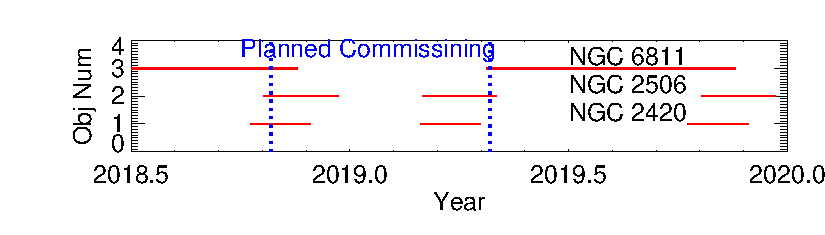
\includegraphics[width=.4\columnwidth]{cluster_visibilty.pdf}
\caption{Visibility windows for the three open clusters considered in this report.
The planned commissioning period is shown with vertical blue dashed lines.}\label{fig:clusterVis}
\end{figure}

After selecting the sources, we discovered that the WEBDA database had parameters that were significantly different from the literature for these individual clusters.
For example E(B-V) = 0.16 for NGC 6811 whereas \citet{molendaz2016spec6811} has E(B-V) = 0.05.
We therefore did a literature search for the most recent available cluster parameters.
Table \ref{tab:clusterProp} shows the properties gathered from the literature.
The most up-to-date literature values indicate that all three clusters have low extinction with E(B-V) $<$ 0.1.
Including uncertainties, the extinctions are actually all consistent with 0.06, but it should be noted that the NGC 2506 uncertainties are likely underestimated since their were derived from a standard error of the mean and may not include systematics.

\begin{table}
\centering
\caption{Cluster Parameters}\label{tab:clusterProp}
\begin{tabular}{lrrrc}
\hline \hline
Cluster   					&  E(B-V) 			& Distance Mod 	& [Fe/H] 			& Age \\
          					&     				&    (m - M)$_V$	& 	dex 			& Gyr \\
\hline \hline
NGC 2420\tablenotemark{a}	& 0.04 $\pm$0.03	&  11.88 $\pm$ 0.27	& -0.05 $\pm$ 0.03	& 3 $\pm$ 1 \\
NGC 2506\tablenotemark{b}	& 0.058 $\pm$ 0.001	&  12.75 $\pm$ 0.10 	& -0.32 $\pm$ 0.03	& 1.85 $\pm$ 0.05 \\
NGC 6811\tablenotemark{c}	& 0.05 $\pm$0.02	& 10.29 $\pm$ 0.14	& 0.04 $\pm$ 0.01 	& 1.0 $\pm$ 0.1 \\
\hline
\end{tabular}
%\caption{G2V-type star saturation K band limits are shown for suggested sub-array sizes. The size affects the number of DHS that can be included, so the noise in the DHS spectra over 1.1 -- 1.9$\mu$m at the given saturation limit for a 1 hour transit is shown in column 4 at native R $\sim$ \DHSresApprox\ resolution.}\label{tab:SatSNRsubA}
\tablenotetext{a}{NGC 2420 parameters from \citet{pancino2010chem2420}.}
\tablenotetext{b}{NGC 2506 parameters from \citet{anthonytwarog2016wiyn2506}. Error bars are formal standard errors of the mean, not necessarily capturing systematics.}
\tablenotetext{c}{NGC 6811 parameters from \citet{molendaz2016spec6811}}
\end{table}

\section{Pan-Starrs}
\subsection{Pan-Starrs Photometry}

We obtained $grizy$ Pan-Starrs photometry \citep{magnier2013photLadder,schlafly2012photcal,tonry2012panstarrsPhot} for all three clusters.
Additionally, we used \citet{janes2013keplerPhot} B and V photometry for NGC~6811 which is in the Kepler field because there were more faint source detections.
We also estimated the Pan-Starrs $g$ - $r$ and B-V colors from a Pickles G2~V spectrum using \texttt{pysynphot} \citep{lim2015pysynphot}, the measured extinction shown in Table \ref{tab:clusterProp} with a Milky Way Diffuse R(V)=3.1 \citet{cardelli1989} extinction law.
Figure \ref{fig:cmdPS} shows the Pan-Starrs and \citet{janes2013keplerPhot} color magnitude diagram for the three clusters along with vertical bars with the expected solar color for each cluster: $g-r$ =0.42, $g-r$ = 0.43 and B-V = 0.67 for NGC~2420, NGC~2506 and NGC~6811 respectively.
Note that the initial selection of NGC~2420 stars ignored the small extinction and put a higher priority on stars bluer than solar.

\begin{figure*}[!t]
\centering
\subfloat[NGC 2420]{
	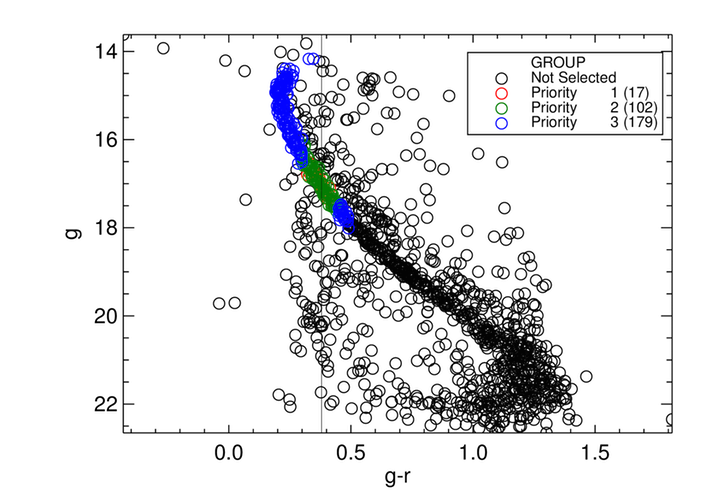
\includegraphics[width=0.5\textwidth]{sources_ngc2420.png}
	\label{fig:cmdNGC6811}
	}
\subfloat[NGC 2506]{
	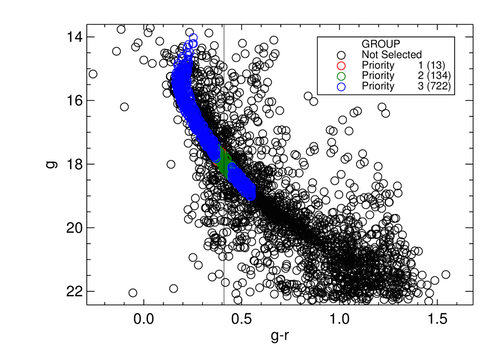
\includegraphics[width=0.5\textwidth]{sources_ngc2506.png}
	\label{fig:cmdNGC2506}
	}
\\
\subfloat[NGC 6811]{
	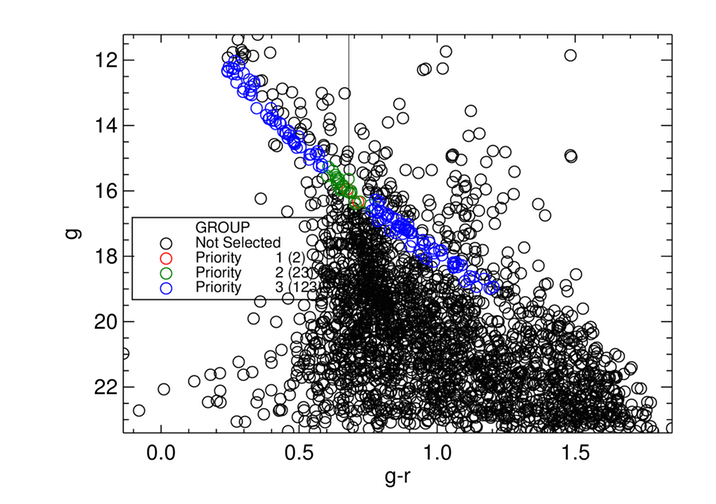
\includegraphics[width=0.5\textwidth]{sources_ngc6811.png}
	\label{fig:cmdNGC6811}
	}
	\caption{Color-magnitudes of the three clusters.
	The main sequence in each cluster was fit with a polynomial and then three priority levels were chosen for follow-up spectroscopy.
	The first priority targets were near-solar $g-r$ or B-V colors ($\pm 0.04, 0.03, 0.05$) that were within $\pm$4\arcmin\ of the cluster center (to concentrate in the NIRCam field of view).
	The second priority were near-solar $g-r$ or B-V colors but with a wider field of view (1$\degree$) to include G2~V stars that could be observed with larger dithers.
	Thirdly, any remaining main sequence stars that were within the 1$\degree$ hectospec field of view with reasonable signal to noise were selected to allow for errors in photometric color predictions and enable star cluster science at the main sequence turnoff point.}
	\label{fig:cmdPS}
\end{figure*} 

\subsection{UKIRT Photometry}

We observed all three clusters with WFCAM on the UKIRT telescope.
This is the same instrument, pipeline and telescope for the UKIDSS survey.
As recommended by the pipeline team, we used aperture photometry number 3 (1\arcsec\ radius) for the fluxes in the J, H and K bands.

\subsection{Tie-in to 2MASS Photometry}

The stars within the clusters explored will be tied to the measurements of the Sun.
\citet{rieke2008absIRcal} provide recommended adjustments to 2MASS photometry which match well with the Solar spectrum.
We can use existing 2MASS measurements of stars within the UKIRT field of view as a reference for the UKIRT photometry.
There are plenty of sources with 2MASS measurements.
For NGC 2420, for example, there are 300-400 stars within the neighboring arrays and 800 near the cluster (many of which will be contaminated by crowding).

\begin{figure}[!hbtp]
\centering
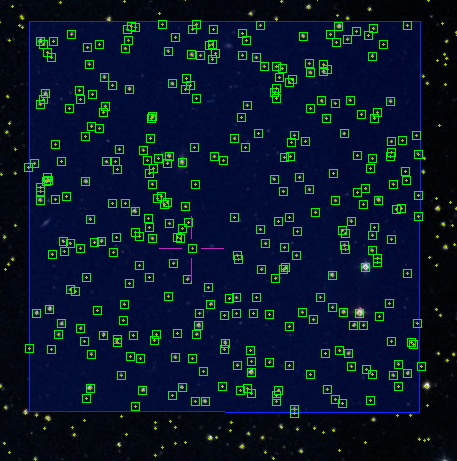
\includegraphics[width=.4\columnwidth]{aladin_ngc2420_wfcam_square.png}
\caption{One of WFCam's 4 detectors near the cluster NGC 2420 which encompasses 315 objects from the 2MASS point source catalog.}\label{fig:wfcam3}
\end{figure}

\section{NIRCam Footprint}
\begin{figure}[!hbtp]
\centering
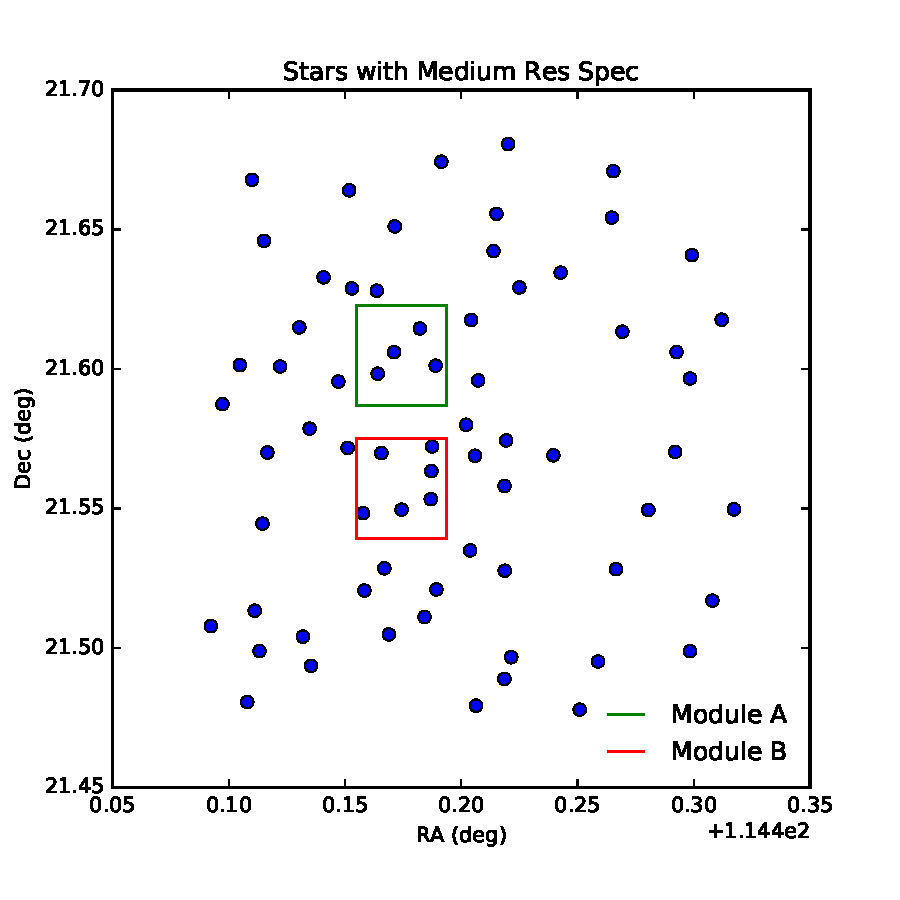
\includegraphics[width=.4\columnwidth]{nircam_fov_fibers.pdf}
\caption{NGC 2420 fibers on the first pass with the FOV of both the A and B modules of NIRCam.
Only 10 stars fit within NIRCam's FOV.}\label{fig:NCFOV}
\end{figure}

\clearpage
\section{Spectral Typing of Candidate Analogs}

\subsection{Hectospec Observations}
We observed NGC~2420 with two fiber configurations in the Spring and Fall of 2016.
We used the 600 gpm grating (1.9 - 2.2 $\AA$ resolution element) to match with existing spectral template libraries with 3.6 $\AA$ resolution.
We selected the central wavelength to be 4800 $\AA$ which means that the wavelength coverage is about 3550 to 6050 $\AA$, which covers several import criteria for G-star classification many of which are concentrated between 4000 and 4400 $\AA$.
We obtained exposure times from 1.2 to 2 hours.
The minimum fiber separation $\sim$20$\arcsec$ required that we observe in two configurations to increase the density of stars for which we had spectral classification.
During the observing run in the Fall of 2016, the 600 gpm (1.9 - 2.2 $\AA$ resolution element) grating had to be removed for fixing and so we were forced to observe NGC 2506 with the 270 gpm (4.5 - 5.2 $\AA$ resolution element).

The Hectospec instrument on the MMT \citep{fabricant2005hectospec,mink2007hectoFibers} was used to obtain spectra of candidate solar analogs in the clusters .
We processed the data with the standard IDL routine \texttt{HSRED}\footnote{https://www.mmto.org/node/536}, which applies automatic bias and flat field corrections, spectral extraction and wavelength calibration.
\texttt{HSRED} can apply flux calibration for F-type stars, but we elected to rectify the spectra 

We normalized the raw spectra output from \texttt{HSRED} in order to pass it to a spectral rectification program \texttt{mkclass} \citep{gray2014classification}.
The first step in the normalization was to get an approximately normalized curve from the strongly curved spectrum shown in Figure \ref{fig:SpecRect}.
We fit an 8th order polynomial in log space to the flux as a function of wavelength.
It is important to do the fit in log-space because in linear space there are regions (near 3800 $\AA$) where the best-fit polynomial drops to low values and the fit can have zero crossings.
If this polynomial model (fit in linear space) is used to rectify the spectrum, the rectified spectrum will have large negative values or NaNs when divided by the model, whereas the fit in log-space has no zero-crossings and reduced systematics at low fluxes.
The polynomial fit is done piecewise in 3 equally spaced regions to take on small scale curvature.

The second step in the spectral rectification process is to normalize by the pseudo continuum and remove any residual curvature.
This is again fit with an 8th order polynomial in a piecewise fashion in three equally spaced wavelength chunks.
The modification for the second step is to do it in linear space (now that zero crossings will not occur) and also select only points greater than 1.0 to ensure they are continuum points.
The two steps (with polynomial fits) and final resulting spectrum are shown for an example source in Figure \ref{fig:SpecRect}.

\begin{figure}[!hbtp]
\centering
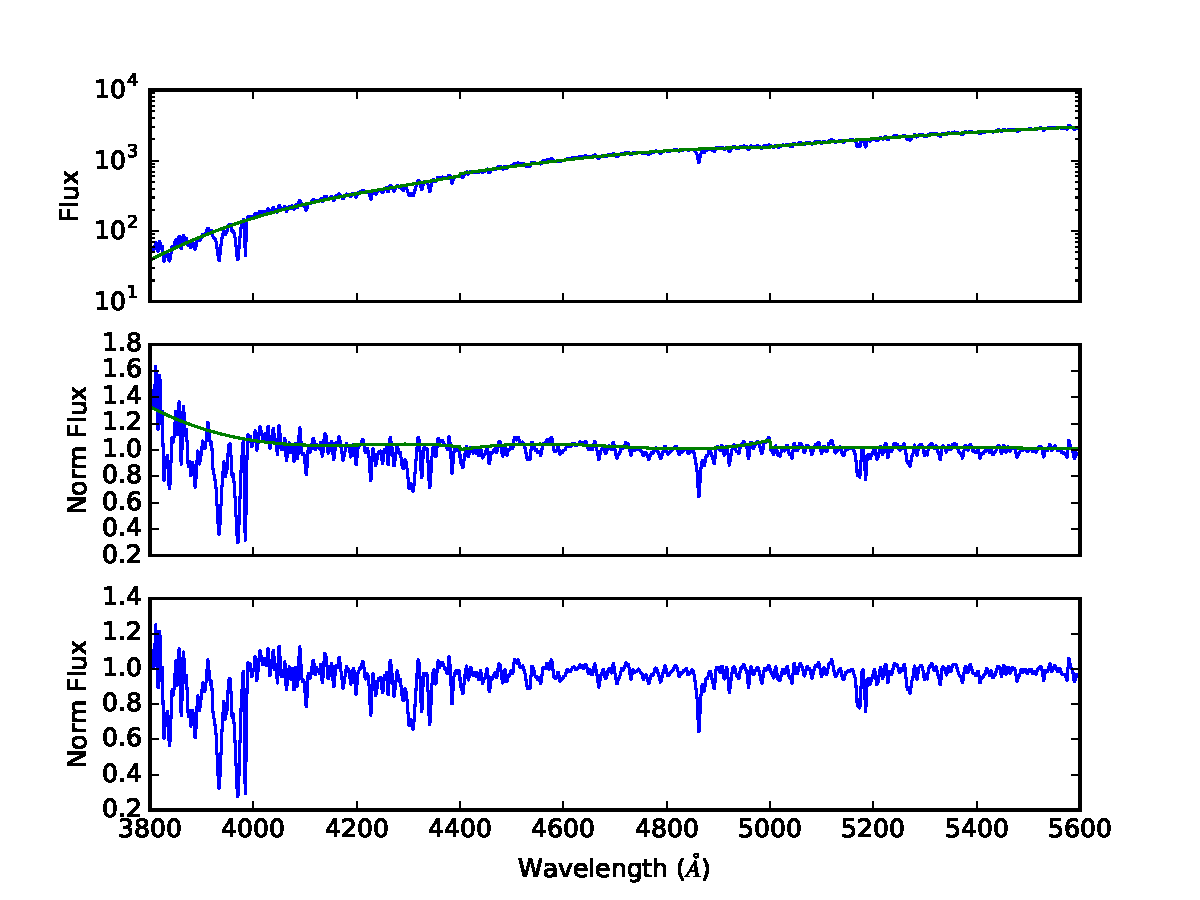
\includegraphics[width=.7\columnwidth]{O_0738209_p2134_rectification.pdf}
\caption{The spectral rectification process happens in two steps 1) take out the strong curvature with a piecewise polynomial in log flux space (top panel) and 2) fit the points above 1.0 with a new piecewise polynomial in linear flux space.
The resulting spectrum is used for classification.}\label{fig:SpecRect}
\end{figure}

\begin{figure}[!hbtp]
\centering
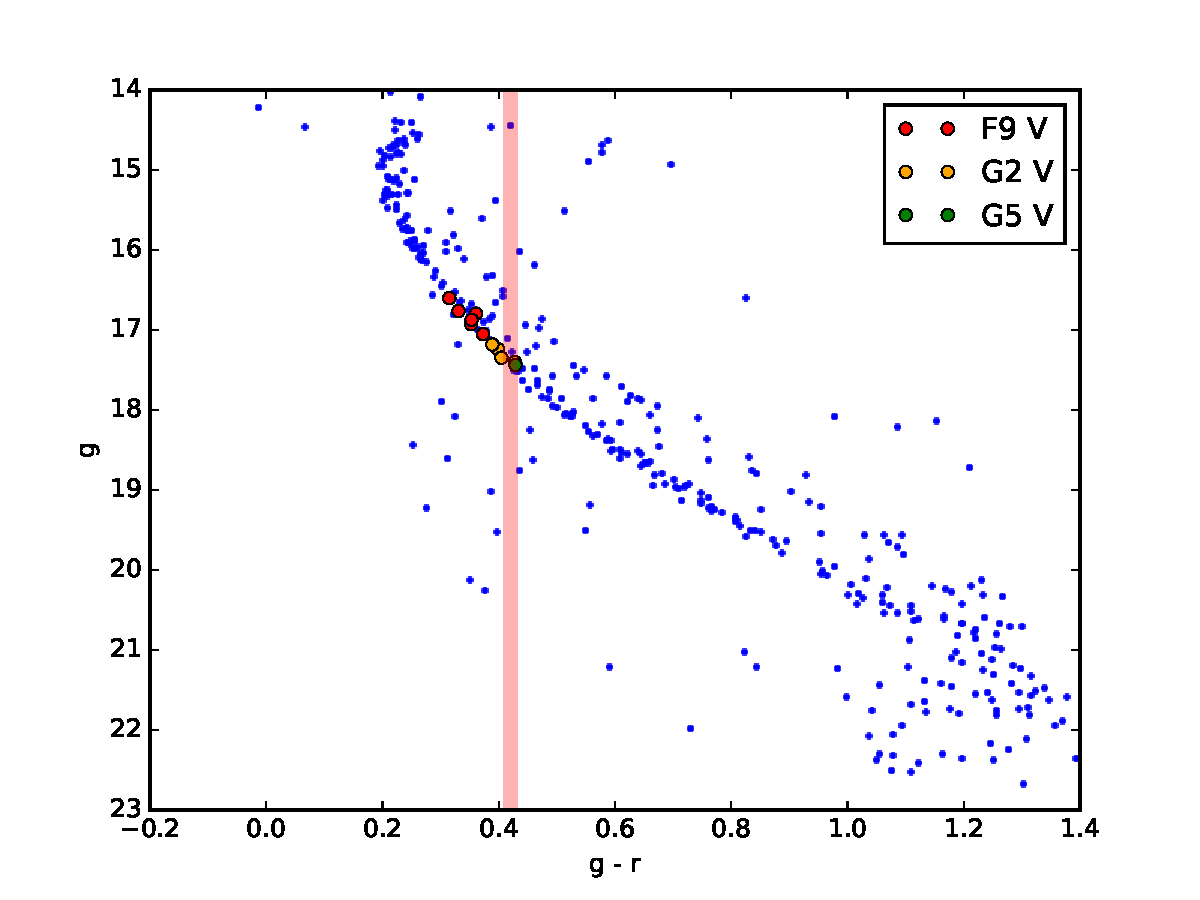
\includegraphics[width=.49\columnwidth]{colormag.pdf}
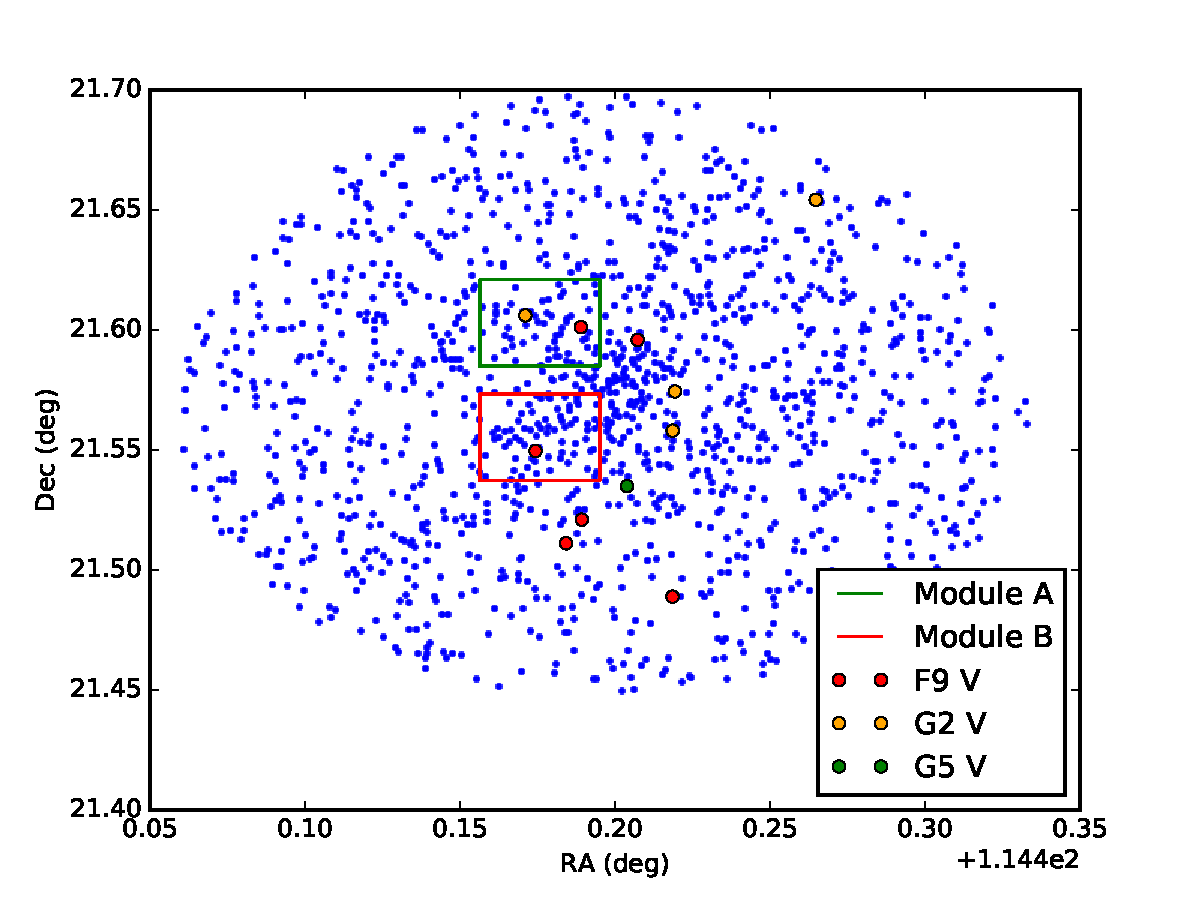
\includegraphics[width=.49\columnwidth]{fov_ngc2420_spTypes.pdf}
\caption{{\it Left} NGC 2420 color magnitude diagram with G2 V stars identified from classification. {\it Right} Field of view with NIRCam footprint.}\label{fig:NCFOV}
\end{figure}

Figure \ref{fig:NCFOV} shows the photometry and positions of sources after 1 pass with Hectospec/MMT and Figure \ref{fig:NCFOV2ndrun} shows after a 2nd set of observations with Hectospec/MMT.

\begin{figure}[!hbtp]
\centering
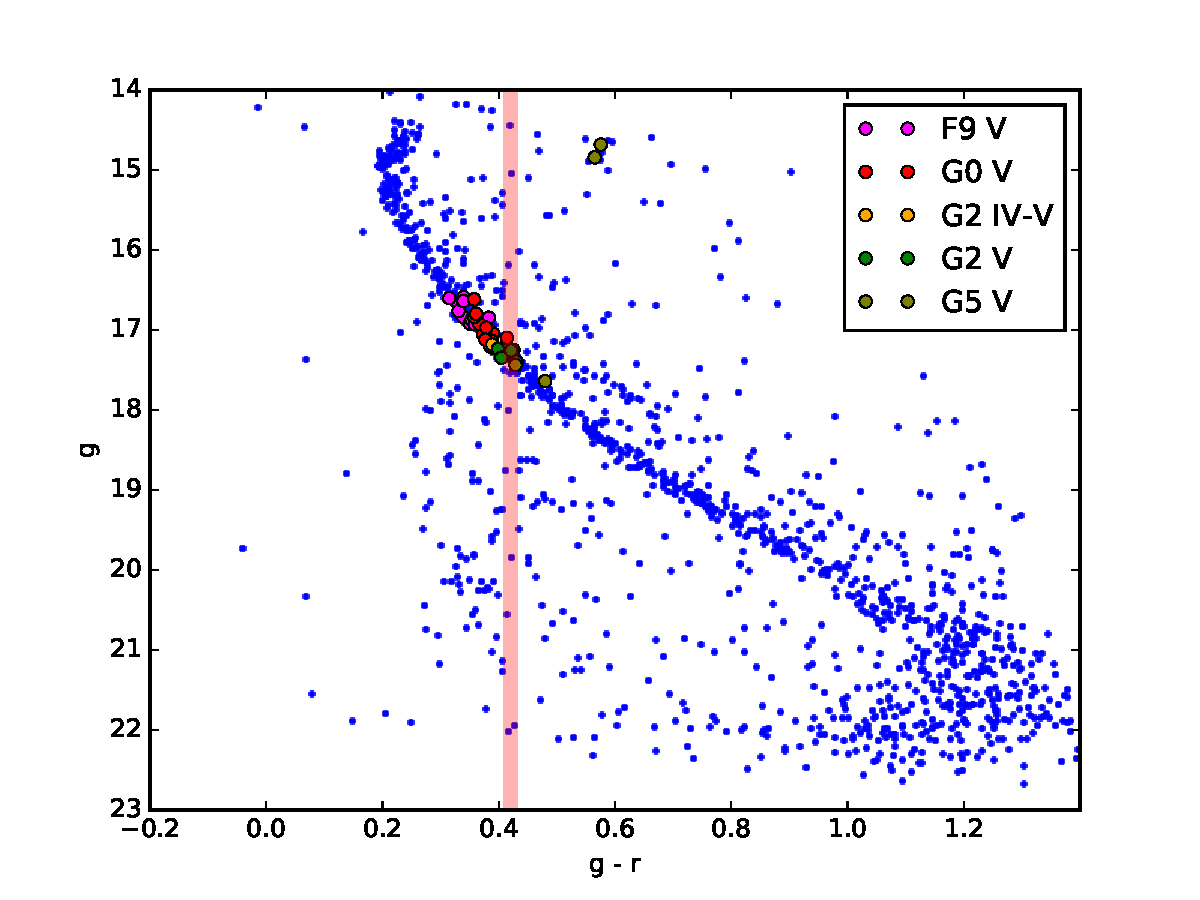
\includegraphics[width=.49\columnwidth]{colormag_two_runs.pdf}
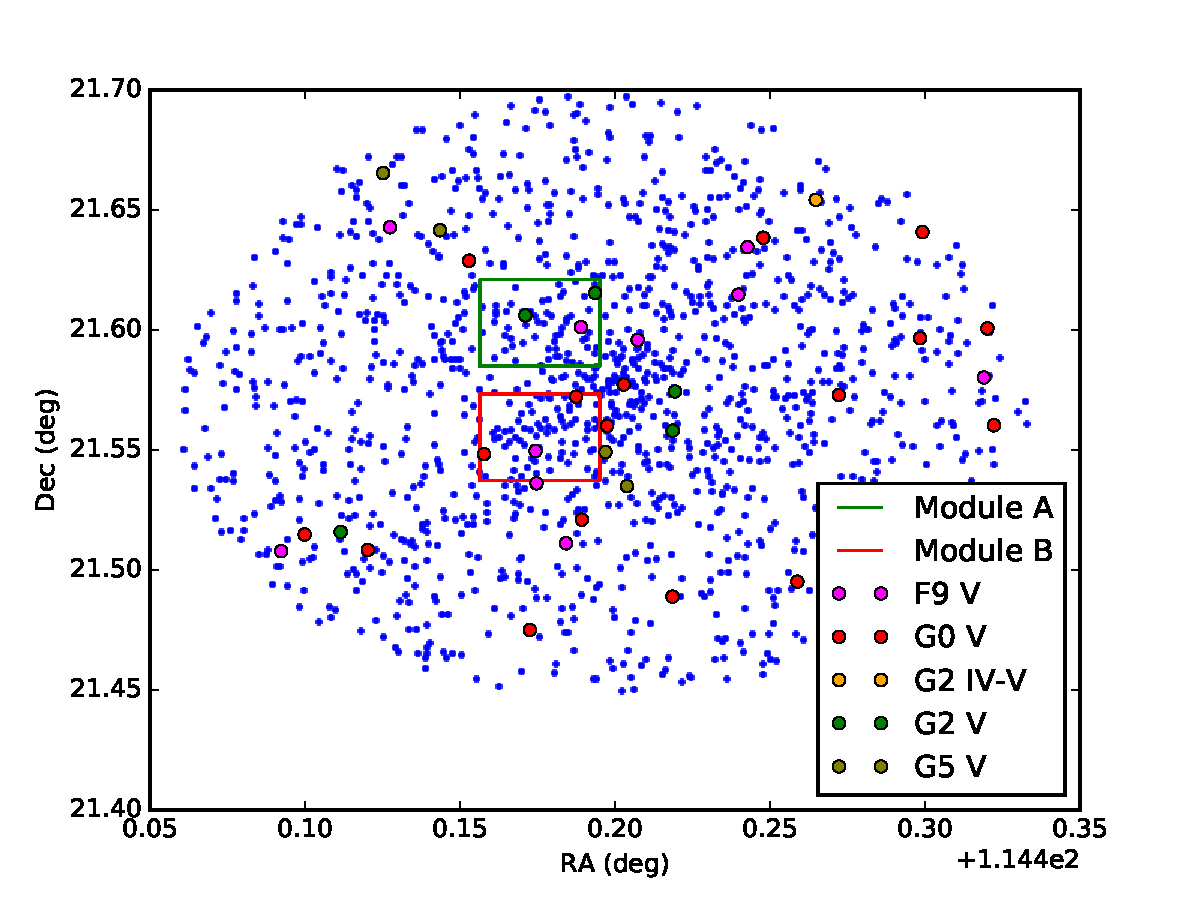
\includegraphics[width=.49\columnwidth]{fov_ngc2420_two_runs.pdf}
\caption{We observed additional stars with Hectospec on the MMT search for additional G2~V sources. This shows the same plot as Figure \ref{fig:NCFOV} after a second Hectospec fiber configuration.
{\it Left} NGC 2420 color magnitude diagram with G2 V stars identified from classification. {\it Right} Field of view with NIRCam footprint.}\label{fig:NCFOV2ndrun}
\end{figure}

\clearpage

\section{Transferring to Directly Calibrated Sources - the NIRCam Flux Ladder}

The primary JWST standards for absolute calibration have been tied to directly calibrated photometric sources through transfers, such as with HST's STIS instrument.
As an independent check on those transfers, NIRCam can be used to observe directly calibrated stars (such as the MSX calibrators \citep{price2004msxCal}) and step down in brightness to faint standards used in JWST calibration.
Figure \ref{fig:sensitivityLadder} shows a schematic of the steps beginning with Midcourse Survey Experiment (MSX) calibrators (as bright as $K \sim -3$) to faint JWST standards ($K \sim 16$).

\begin{figure}[!t]
\centering
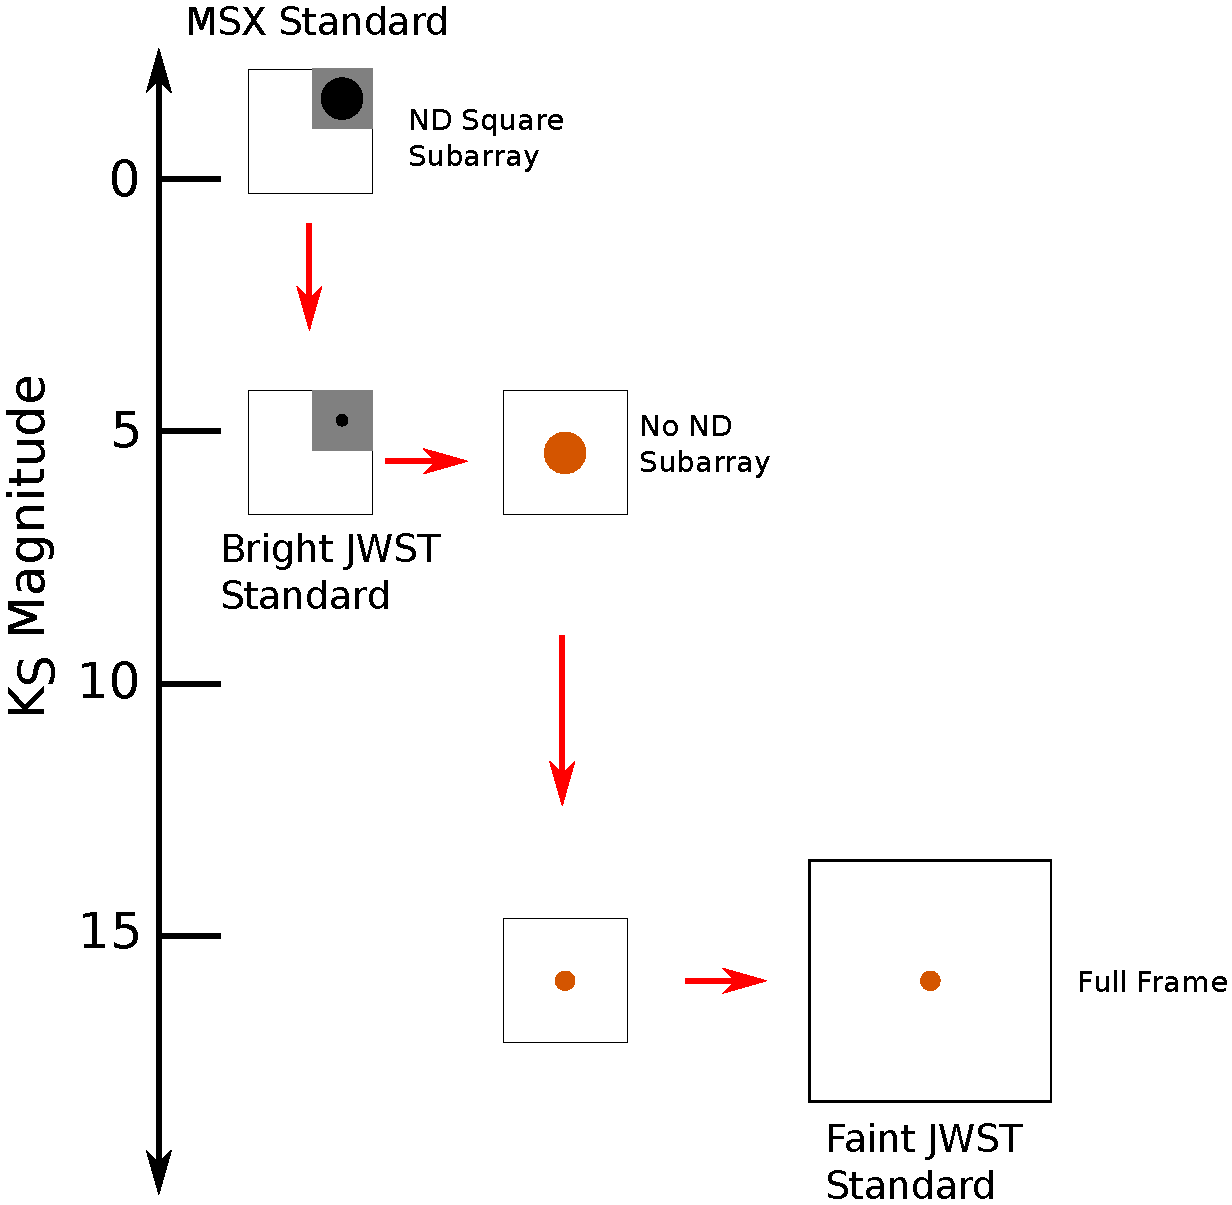
\includegraphics[width=.55\columnwidth]{flux_ladder.pdf}
\caption{Schematic sensitivity ladder going from an MSX standard (with a sub-array, neutral density filter observation) to a faint JWST standard (with a full array, full throughput observation).
An intermediate standard can be used to check the NIRCam transfers against other observatories and instruments.}\label{fig:sensitivityLadder}
\end{figure}

\begin{table}[!b]
\centering
\caption{Conversion from Directly Calibrated Source to Deep Calibrator}\label{tab:conversionSteps}
\begin{tabular}{lrrrrrrrr}
\hline \hline
Step		& Source						& Spectral Type	& $K_\mathrm{src}$		& ND Square		& Subarray	& Filter & t$_\mathrm{exp} (s) $ &$K_\mathrm{sat}$\\
\hline \hline
1		& MSX Calibrator\tablenotemark{a}	& A1 V to M0 III		& -3 to 0.1		& On	&	64$\times$64	& F430M &  0.2 & -4.0 \\
2		& Bright JWST Calibrator			& G2 V			& 6.5	  		& On &	64$\times$64	& F430M &  220 & -4.0 \\
3		& Bright JWST Calibrator			& G2 V			& 6.5  		& Off &	64$\times$64	& F430M &  0.1 & 6.2 \\
4		& Faint JWST Calibrator			& G2 V			& 16 			& Off &	64$\times$64	& F430M &  94 & 6.2 \\
5		& Faint JWST Calibrator			& G2 V			& 16 			& Off &	Full Frame	& F430M &  107 & 12 \\
6		& Faint JWST Calibrator			& G2 V			& 16 			& Off &	Full Frame  	& F444W &  21 & 13.7 \\
\hline
\end{tabular}
\tablenotetext{a}{Any directly calibrated bright source such as the MSX calibrators \citep{price2004msxCal}, (which include Sirius and Vega) or alternatively $\alpha$ Cen A. The exposure times given are the times needed to reach at least SNR=200, rounded up to the next group up the ramp. The saturation limit is the 80\% well depth for 2 non-destructive reads up the ramp following a reset.}
\vspace{0.05in}
\end{table}

The methodology of the flux ladder is that only one change is made per step - either an instrument re-configuration is made on the same source or a new source is measured with the same instrument configuration.
As listed in Table \ref{tab:conversionSteps}, the direct calibrator would be observed in a neutral density square, subarray and medium band filter while using the coronagraphic pupil.
For the next step, this same instrument configuration will be used on a bright JWST standard, such as HD 37962 (G2 V, $K$=6.27).
Getting sufficient signal to noise (S/N$\gtrsim$200) on an intermediate JWST calibrator such as P-330E (G2 V, $K$=11.4) with the neutral density square in place would require unfeasibly long integration times so the bright calibrators are preferred for steps 2 and 3.

This bright JWST standard would be used to transfer from the ND filter with a coronagraphic pupil mask to direct imaging.
This conversion step can independently be checked against other instruments' measurements of the bright JWST calibrator, such as by STIS with HST.
The next step would be to use the same direct image configuration and subarray size to observe a faint JWST calibrator around $K \sim$15.
S/N ratios of 200 can be achieved in 94 seconds in this mode.
This calibrator star would now be observable in full frame mode without saturation so the next step would be a conversion from subarray to full frame on the same source.
To calibrate the wide band filters, such as F444W, one final step would be needed to go from the medium to wide band photometry using a model for the star.
Either a well-characterized white dwarf spectrum of a known standard or a faint G2 V standard from an open cluster would be good models for this transfer of filters.

Figure \ref{fig:sensitivityLadder} shows that an intermediate JWST standard such as P-330 E can be used to check transfers and detector linearity corrections.
This step would not be a ``rung'' in the NIRCam flux ladder since it would require more transfers to achieve the last step of full frame wide band imaging, but serves as another check on the transfers from bright to faint targets.

\subsection{Ways to Observe Bright Stars}\label{sec:brightStarMode}

There are several ways to improve saturation limits with NIRCam over direct imaging:
\begin{itemize}
\item \textbf{Lyot Stop} Cut down the aperture size with a Lyot stop. These have 19\% throughput (1.8 mags). Additionally, this broadens the PSF - see Figure \ref{fig:psfComparison}.
The broadening spreads light out by a similar factor (contributing 1.8 mags to saturation limits) for a total of 3.5 mags.
\item \textbf{Neutral Density Square} The neutral density filters have an attenuation of 10$^3$ or 7.5 mags. A color correction would have to be applied for the neutral density filter (since it is wavelength dependent) when transferring to an un-occulted region.
Additionally, the Lyot stop that must be in place to use the neutral density filter so the total improvement on saturation limits is 11 mags over direct imaging.
Care must be taken with dithering to ensure that non-uniform optical depth of the neutral density filter doesn't affect the photometry.
\item \textbf{Grisms} For long wavelength NIRCam observations ($2.4~\mu$m$ > \lambda < 5~\mu$m), one can use a grism to spread out the light. This mode still has a saturation limit of $K$=4.6 to 3.5 for the F322W2  filter and 2048$\times$64 subarray \citep{greene2016wfss}, which does not reach to the MSX standards. This could be potentially combined with the coronagraphic pupil, but this combination has been tested or explored in detail. One could potentially observe small pieces of the spectrum at a time with a subarray that are all combined to create a spectrum, but this would add time and may be difficult to implement.
\item \textbf{DHS} For short wavelength NIRCam spectra ($1.0~\mu$m$ > \lambda < 2.0~\mu$m), one can use the Dispersed Hartmann Sensor. The dispersed Hartmann Sensor (DHS) reduces the pupil throughput and spreads the light out to reach saturation limits of $K$=0.2 to 1.5 depending on spectral type \citep{schlawin2017dhs} for a 2048$\times$64 subarray.
This is not bright enough to observe the MSX calibrators.
As with the long wavelength grisms, one would have to read small subarrays (e.g. 64$\times$64) to get to brighter limits.
If one stitched together a spectrum from these subarrays along the spectrum, this could theoretically be used on all MSX stars.
However, the time to build up 32 pieces
\item \textbf{Extra Small Subarrays} There will be an engineering jitter monitoring test with an 8 $\times$ 8 subarray.
There may be complications with calculating accurate integration times in this mode because any uncertainty's affecting a frame time could be a significant fraction of the $\sim$ 2 ms frame time.
The background annulus would be limited for such small subarrays.
\item \textbf{Weak Lens} The Weak Lenses spread light out over many pixels which can be helpful for bright stars. However, one needs to read out larger sized subarrays to encompass the entire hexagonal PSF so this somewhat cancels out the effect of spreading the light out over many pixels.
For a very narrowband filter such as F212N, the K-band saturation limit for a weak lens observation with a 128$\times$128 subarray is 0.9 mag for a G2V star, which does not quite reach the MSX calibrators.
\end{itemize}

Of the many options here, the most feasible method is the neutral density square with the Lyot Coronagraphic pupil mask.
Sensitivity and saturation limits make use of \texttt{pysynphot} \citep{lim2015pysynphot} with either Phoenix stellar models \citep{allard2012phoenix} or \citet{castelli2004models} models.

\subsection{Tie-in to MSX}

Figure \ref{fig:msxNCfilterOverlap} shows the MSX filters B1 and B2 as compared to the NIRCam long wavelength filters -- we only include filters that have some overlap.
The F430M filter is the best match with the MSX bands.
Figure \ref{fig:msxNCfilterOverlap} also shows model spectra from \citet{castelli2004models} for the MSX calibrator stars in \citet{price2004msxCal} near these bandpasses.
The flux has been normalized for each star at 3.6~$\mu$m and then offset for clarity.
We use the nearest match between the stellar types from the Simbad database and the suggested \citet{castelli2004models} parameters.\footnote{http://www.stsci.edu/hst/observatory/crds/castelli\_kurucz\_atlas.html}

Observing these bright sources (which are bright naked eye stars) with JWST's NIRCam can be achieved with a combination of medium-band filters, small subarray sizes, a Lyot stop pupil mask (19\% transmission) and a neutral density (ND) filter.
Using \texttt{webbpsf} and the throughputs in a NIRCam program called \texttt{pynrc}, we calculate the saturation limits for 2 groups in RAPID mode and find a K-magnitude of saturation of $-$4.0 for an A1 V type star (Sirius is A1 V with K=$-$1.35) and $-$3.7 for an M3 III (Gacrux is $-$3.12).
This means that the entire sample of stars from \citet{price2004msxCal} are observable in this coronagraphic neutral density mode.

\begin{figure}[!hbtp]
\centering
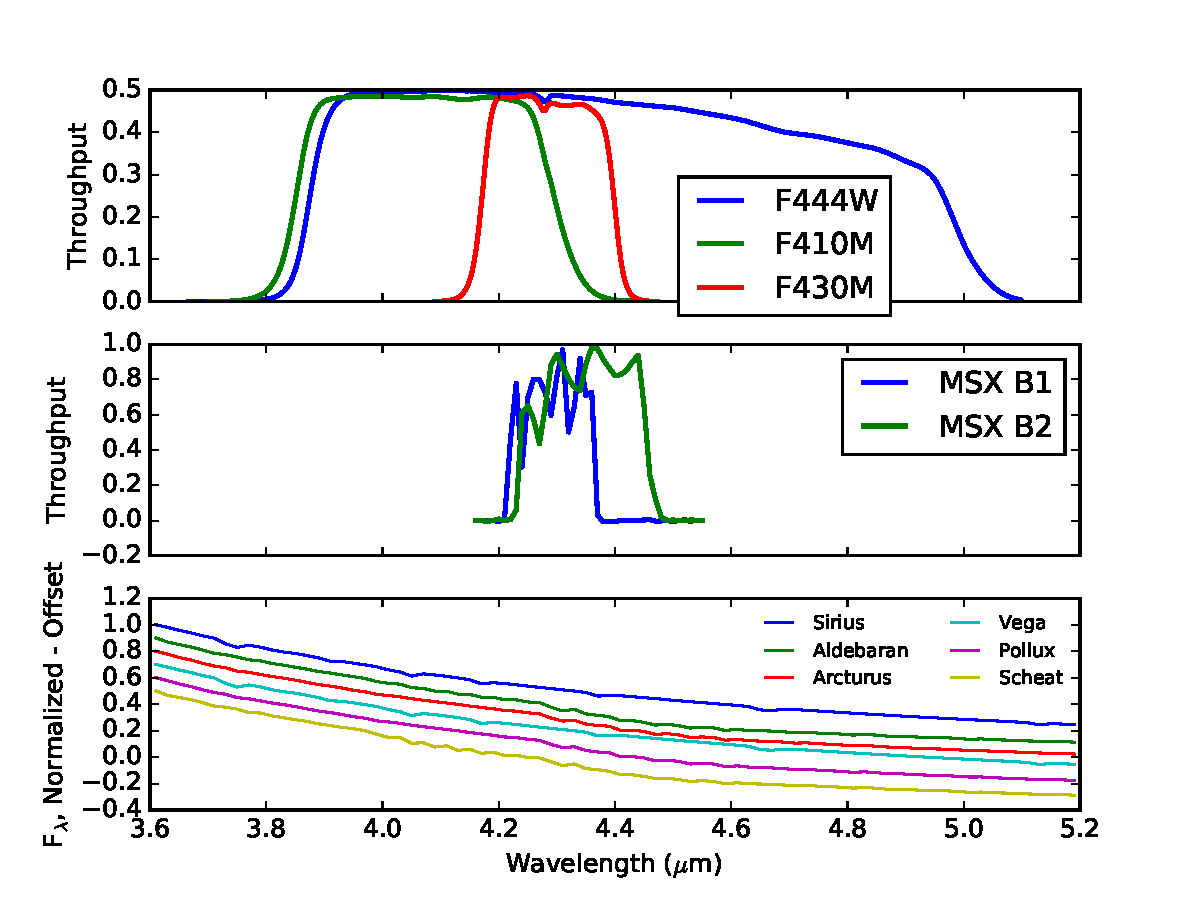
\includegraphics[width=.55\columnwidth]{msx_nircam_filt.pdf}
\caption{NIRCam filter throughputs (top), MSX filter throughputs \citep{egan1999msxGuide} (middle) and model spectra of MSX calibrator stars (bottom). F430M best matches the MSX filters.}\label{fig:msxNCfilterOverlap}
\end{figure}

\subsubsection{Complications with PSF}
A Lyot pupil mask must be used when imaging through the neutral density squares since the wedges that redirect light through NIRCam's coronagraphic masks and neutral density squares are co-located with the Lyot stop pupil masks.
In addition to lowering the transmission by a factor of 0.19\%, the Lyot stops spread out the PSF as compared to direct imaging.
Figure \ref{fig:psfComparison} shows example PSFs calculated with \texttt{webbpsf} \citep{perrin2012webbpsf}.
Figure \ref{fig:psfDirect} shows the direct image PSF versus the the coronagraphic PSF (Figure \ref{fig:psfND}), both normalized to the peak pixel.

When using the ND filter and Lyot stop, the aperture photometry must account for the large secondary peaks of the PSF.
This can be accomplished with a large aperture covering all the secondary peaks assuming that the background levels are low and that there are no nearby sources.
Alternatively, one could extract the flux from the core of the PSF.

\begin{figure*}
\centering
\subfloat[Direct Imaging PSF]{
	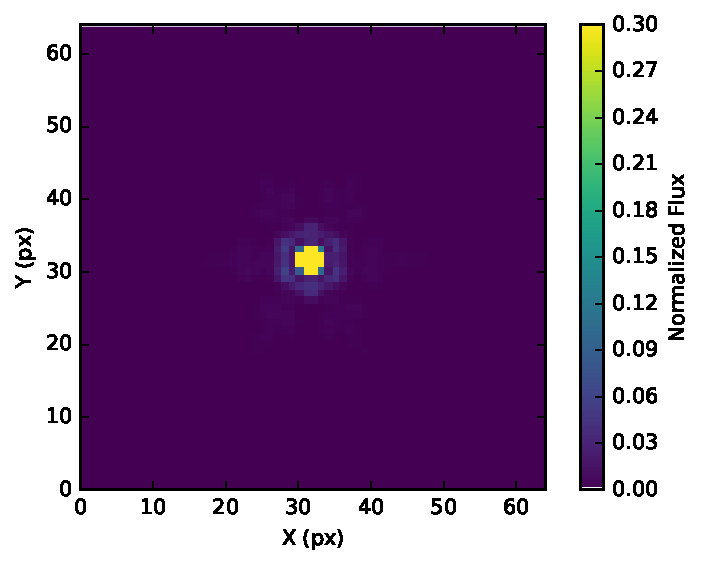
\includegraphics[width=0.45\textwidth]{psf_direct.pdf}
	\label{fig:psfDirect}
	}
\subfloat[NGC 2506]{
	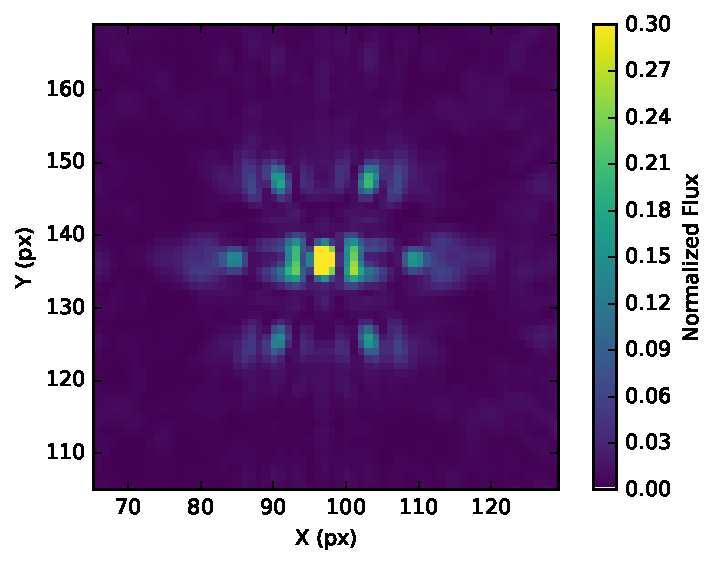
\includegraphics[width=0.45\textwidth]{psf_ND.pdf}
	\label{fig:psfND}
	}
	\caption{The \texttt{webbpsf} direct imaging PSF and coronagraphic PSF which is modified by the Lyot stop. Both images are normalized by the peak pixel value and have arbitrary array positions but the same height and width. Aperture photometry of the sources imaged through the coronograph will have to use a large aperture encompassing the 6 outer peaks or just use the central peak(s) and apply careful background subtraction. Both PSFs were calculated for NIRCam's long wavelength channel with a F430M filter.}
	\label{fig:psfComparison}
\end{figure*} 

\subsubsection{Complications with Flat Fielding}
The ND filters are not uniform spatially.
Correcting for any pinholes or blemishes in the ND square surface will likely dominate the error budget for the ND square absolute calibration.
Positioning the sources consistently on the same pixel locations and using the same dither patterns will help with these errors.
The dithers can be used to check the surface irregularities.

\subsubsection{Clocking Issues for Small Subarrays}

Marcia and Jarron have brought up this issue in a NIRCam STScI+External team telecon on on April 6, 2017.
This is a known bug in the ASIC micro-code that can affect the integration times of small subarrays.
There are sometimes unpredictable frames which will have an additional row time (so a 1/64) increase in frame time.
This could potentially decrease the flux by 1.6\% so it is a concern for flux calibration, but it is also a rare occurrence, happening for 5 frames out of 8000.
Multiple exposures and dither positions should help lessen this effect, especially if averaged with robust statistics.

\section*{Acknowledgements}
%\acknowledgments

Thanks to Daniel Kiminki and John Stauffer for the selection of open clusters for this work and for finding targets based on initial data.
Thanks to Richard Gray and Chris Corbally for their help in stellar classification and guidance with the Hectospec observations.
Funding for the NIRCam team is provided by NASA Goddard Spaceflight Center. This research has made use of the WEBDA database, operated at the Department of Theoretical Physics and Astrophysics of the Masaryk University.
Observations reported here were obtained at the MMT Observatory, a joint facility of the University of Arizona and the Smithsonian Institution.
This paper uses data products produced by the OIR Telescope Data Center, supported by the Smithsonian Astrophysical Observatory.
The Pan-STARRS1 Surveys (PS1) have been made possible through contributions of the Institute for Astronomy, the University of Hawaii, the Pan-STARRS Project Office, the Max-Planck Society and its participating institutes, the Max Planck Institute for Astronomy, Heidelberg and the Max Planck Institute for Extraterrestrial Physics, Garching, The Johns Hopkins University, Durham University, the University of Edinburgh, Queen's University Belfast, the Harvard-Smithsonian Center for Astrophysics, the Las Cumbres Observatory Global Telescope Network Incorporated, the National Central University of Taiwan, the Space Telescope Science Institute, the National Aeronautics and Space Administration under Grant No. NNX08AR22G issued through the Planetary Science Division of the NASA Science Mission Directorate, the National Science Foundation under Grant No. AST-1238877, the University of Maryland, and Eotvos Lorand University (ELTE) and the Los Alamos National Laboratory. 

%If used, some data was collected from the Open Exoplanet Catalogue \citep{rein2012openExoCat}.

%% In a manner similar to \objectname authors can provide links to dataset
%% hosted at participating data centers via the \dataset{} command.  The
%% second curly bracket argument is printed in the text while the first
%% parentheses argument serves as the valid data set identifier.  Large
%% lists of data set are best provided in a table (see Table 3 for an example).
%% Valid data set identifiers should be obtained from the data center that
%% is currently hosting the data.
%%
%% Note that AASTeX interprets everything between the curly braces in the 
%% macro as regular text, so any special characters, e.g. "#" or "_," must be 
%% preceded by a backslash. Otherwise, you will get a LaTeX error when you 
%% compile your manuscript.  Special characters do not 
%% need to be escaped in the optional, square-bracket argument.



%% In this section, we use  the \subsection command to set off
%% a subsection.  \footnote is used to insert a footnote to the text.

%% Observe the use of the LaTeX \label
%% command after the \subsection to give a symbolic KEY to the
%% subsection for cross-referencing in a \ref command.
%% You can use LaTeX's \ref and \label commands to keep track of
%% cross-references to sections, equations, tables, and figures.
%% That way, if you change the order of any elements, LaTeX will
%% automatically renumber them.

%% This section also includes several of the displayed math environments
%% mentioned in the Author Guide.


%% The equation environment wil produce a numbered display equation.


%% The \notetoeditor{TEXT} command allows the author to communicate
%% information to the copy editor.  This information will appear as a
%% footnote on the printed copy for the manuscript style file.  Nothing will
%% appear on the printed copy if the preprint or
%% preprint2 style files are used.

%% The eqnarray environment produces multi-line display math. The end of
%% each line is marked with a \\. Lines will be numbered unless the \\
%% is preceded by a \nonumber command.
%% Alignment points are marked by ampersands (&). There should be two
%% ampersands (&) per line.

%% Putting eqnarrays or equations inside the mathletters environment groups
%% the enclosed equations by letter. For instance, the eqnarray below, instead
%% of being numbered, say, (4) and (5), would be numbered (4a) and (4b).
%% LaTeX the paper and look at the output to see the results.

%% This section contains more display math examples, including unnumbered
%% equations (displaymath environment). The last paragraph includes some
%% examples of in-line math featuring a couple of the AASTeX symbol macros.

%% The displaymath environment will produce the same sort of equation as
%% the equation environment, except that the equation will not be numbered
%% by LaTeX.
%% If you wish to include an acknowledgments section in your paper,
%% separate it off from the body of the text using the \acknowledgments
%% command.

%% Included in this acknowledgments section are examples of the
%% AASTeX hypertext markup commands. Use \url without the optional [HREF]
%% argument when you want to print the url directly in the text. Otherwise,
%% use either \url or \anchor, with the HREF as the first argument and the
%% text to be printed in the second.

%\acknowledgments



%% To help institutions obtain information on the effectiveness of their
%% telescopes, the AAS Journals has created a group of keywords for telescope
%% facilities. A common set of keywords will make these types of searches
%% significantly easier and more accurate. In addition, they will also be
%% useful in linking papers together which utilize the same telescopes
%% within the framework of the National Virtual Observatory.
%% See the AASTeX Web site at http://aastex.aas.org/
%% for information on obtaining the facility keywords.

%% After the acknowledgments section, use the following syntax and the
%% \facility{} macro to list the keywords of facilities used in the research
%% for the paper.  Each keyword will be checked against the master list during
%% copy editing.  Individual instruments or configurations can be provided 
%% in parentheses, after the keyword, but they will not be verified.

%{\it Facilities:} \facility{Nickel}, \facility{HST (STIS)}, \facility{CXO (ASIS)}.

%% Appendix material should be preceded with a single \appendix command.
%% There should be a \section command for each appendix. Mark appendix
%% subsections with the same markup you use in the main body of the paper.

%% Each Appendix (indicated with \section) will be lettered A, B, C, etc.
%% The equation counter will reset when it encounters the \appendix
%% command and will number appendix equations (A1), (A2), etc.



%% The reference list follows the main body and any appendices.
%% Use LaTeX's thebibliography environment to mark up your reference list.
%% Note \begin{thebibliography} is followed by an empty set of
%% curly braces.  If you forget this, LaTeX will generate the error
%% "Perhaps a missing \item?".
%%
%% thebibliography produces citations in the text using \bibitem-\cite
%% cross-referencing. Each reference is preceded by a
%% \bibitem command that defines in curly braces the KEY that corresponds
%% to the KEY in the \cite commands (see the first section above).
%% Make sure that you provide a unique KEY for every \bibitem or else the
%% paper will not LaTeX. The square brackets should contain
%% the citation text that LaTeX will insert in
%% place of the \cite commands.

%% We have used macros to produce journal name abbreviations.
%% AASTeX provides a number of these for the more frequently-cited journals.
%% See the Author Guide for a list of them.

%% Note that the style of the \bibitem labels (in []) is slightly
%% different from previous examples.  The natbib system solves a host
%% of citation expression problems, but it is necessary to clearly
%% delimit the year from the author name used in the citation.
%% See the natbib documentation for more details and options.

\bibliographystyle{apj}
\bibliography{abscal_biblio}

\clearpage
\pagebreak

\appendix

\section{Notes to Self}

\subsection{Notes on using \texttt{mkclass}}

\subsubsection{Code System}
The library is organized into files like \texttt{t130l50p00.rbn}.
The \texttt{t130} specifies 10 $\times$ the class coding system of O3 through M9 visible in the code \texttt{code3spt.c}.
In this case, \texttt{t130} means code 13.0 and type B7.
The luminosity class is next \texttt{l50} means V.
We use the \texttt{libnor36} library, which appears to work with the "Roughtype 2" method for non-rectified data.
The code runs into segmentation faults if attempting Roughtype 1 with the \texttt{libnor36} library.


\subsubsection{Backgrounds}

Zodiacal background is expressed as a function of the minimum zodiacal background in \texttt{pynrc}.
From the code documentation: average across the sky has zfact = 2.5.
In these models solar B-V=0.65 for 1~M$_\odot$ at 4.25 Gyr.

\subsection{Isochrones}

As a check on the maximum age, I downloaded Dartmouth Isochrones \citep{dotter2008dartmouth} and plotted the color-magnitude diagram in Figure \ref{fig:isochrones}.
At 7 Gyr, the main sequence turnoff begins affecting the selection of stars near solar B-V.
Nearly all open clusters are young ($\lesssim$ 5 Gyr) so this really only affects just NGC 188 \citep[7.1 Gyr][]{elsanhoury2016ngc188}.

\begin{figure}[!hbtp]
\centering
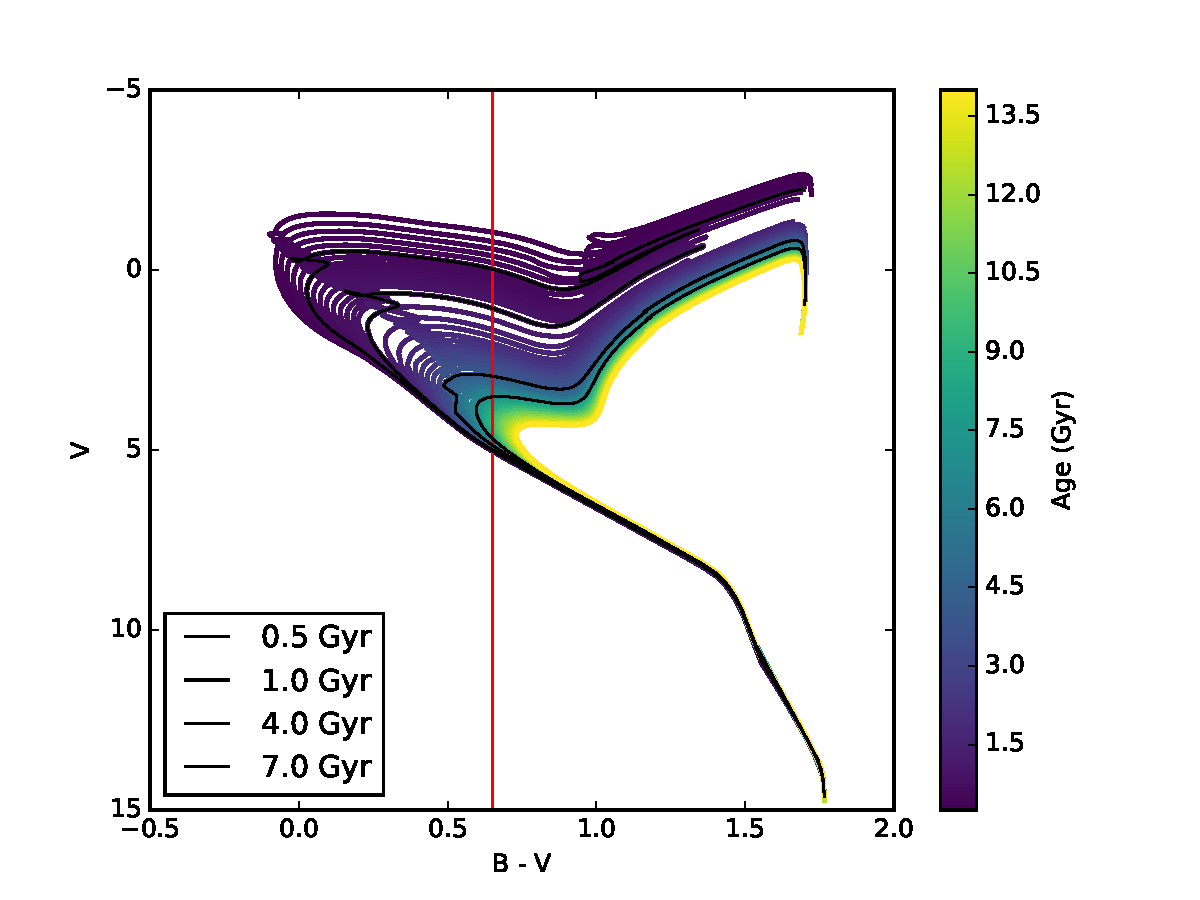
\includegraphics[width=.7\columnwidth]{hr_isochrones.pdf}
\caption{The Dartmouth isochrones \citep{dotter2008dartmouth}, for [Fe/H]=0, show that the age of the cluster should be $\lesssim 7 $Gyr before main sequence turnoff should begin to affect the identification of solar analogs.
The red vertical line represents solar B-V.}\label{fig:isochrones}
\end{figure}

\subsection{UKIRT Calibration}

Our WFCAM data should be calibrated in a similar was as UKIDSS.
Eiichi Egami says we can use the Viking Survey as an independent check on the UKIDSS flux calibration.

\subsection{Sections to Expand in this Report}

George has some requests for this report.
Consider adding notes on calibration of two more instruments.
The solar spectrum is very well measured at infrared wavelengths, so it may be the best one for interpolation from optical/NIR into Far IR.
\begin{enumerate}
	\item MIRI: For the shorter wavelength MIRI bands (say F560W and F770W) photometry, George would like to observe the NIRCam faint G2V stars in order to have a sample of stars that have a highly accurate solar model
	\item NIRSpec: We'd also want to test calibration of NIRSpec w/ our solar G2 V stars.
George recommends the IFU or slits as opposed to MSA because it's less sensitive to positional accuracy.
Note that we would only get 1 G2V star at a time.
Also, beware that no bright stars from the cluster contaminate the field. MSA shutters that are stuck open may introduce significant amounts of stray light.
\end{enumerate}
Note, that George has two concerns about white dwarfs:
\begin{enumerate}
	\item debris disks emission - they have found that magnetic field trapping of dust around A stars can cause excess emission.
White dwarfs have strong magnetic fields and could also trap nano-grain dust.
George and Andras will probably write a paper on white dwarf dust in Fall of 2017.
	\item uncertainties in the IR - white dwarfs don't have a lot of measurements in the IR.
How can we be sure the models are good in the infrared?
\end{enumerate}



%% Use the figure environment and \plotone or \plottwo to include
%% figures and captions in your electronic submission.
%% To embed the sample graphics in
%% the file, uncomment the \plotone, \plottwo, and
%% \includegraphics commands
%%
%% If you need a layout that cannot be achieved with \plotone or
%% \plottwo, you can invoke the graphicx package directly with the
%% \includegraphics command or use \plotfiddle. For more information,
%% please see the tutorial on "Using Electronic Art with AASTeX" in the
%% documentation section at the AASTeX Web site, http://aastex.aas.org/
%%
%% The examples below also include sample markup for submission of
%% supplemental electronic materials. As always, be sure to check
%% the instructions to authors for the journal you are submitting to
%% for specific submissions guidelines as they vary from
%% journal to journal.

%% This example uses \plotone to include an EPS file scaled to
%% 80% of its natural size with \epsscale. Its caption
%% has been written to indicate that additional figure parts will be
%% available in the electronic journal.

%\begin{figure}
%\epsscale{.80}
%\plotone{f1.eps}
%\caption{Derived spectra for 3C138 \citep[see][]{heiles03}. Plots for all sources are available
%in the electronic edition of {\it The Astrophysical Journal}.\label{fig1}}
%\end{figure}

%\clearpage

%% Here we use \plottwo to present two versions of the same figure,
%% one in black and white for print the other in RGB color
%% for online presentation. Note that the caption indicates
%% that a color version of the figure will be available online.
%%

%\begin{figure}
%\plottwo{f2.eps}{f2_color.eps}
%\caption{A panel taken from Figure 2 of \citet{rudnick03}. 
%See the electronic edition of the Journal for a color version 
%of this figure.\label{fig2}}
%\end{figure}

%% This figure uses \includegraphics to scale and rotate the still frame
%% for an mpeg animation.

%\begin{figure}
%\includegraphics[angle=90,scale=.50]{f3.eps}
%\caption{Animation still frame taken from \citet{kim03}.
%This figure is also available as an mpeg
%animation in the electronic edition of the
%{\it Astrophysical Journal}.}
%\end{figure}

%% If you are not including electonic art with your submission, you may
%% mark up your captions using the \figcaption command. See the
%% User Guide for details.
%%
%% No more than seven \figcaption commands are allowed per page,
%% so if you have more than seven captions, insert a \clearpage
%% after every seventh one.

%% Tables should be submitted one per page, so put a \clearpage before
%% each one.

%% Two options are available to the author for producing tables:  the
%% deluxetable environment provided by the AASTeX package or the LaTeX
%% table environment.  Use of deluxetable is preferred.
%%

%% Three table samples follow, two marked up in the deluxetable environment,
%% one marked up as a LaTeX table.

%% In this first example, note that the \tabletypesize{}
%% command has been used to reduce the font size of the table.
%% We also use the \rotate command to rotate the table to
%% landscape orientation since it is very wide even at the
%% reduced font size.
%%
%% Note also that the \label command needs to be placed
%% inside the \tablecaption.

%% This table also includes a table comment indicating that the full
%% version will be available in machine-readable format in the electronic
%% edition.

%% If you use the table environment, please indicate horizontal rules using
%% \tableline, not \hline.
%% Do not put multiple tabular environments within a single table.
%% The optional \label should appear inside the \caption command.



%% If the table is more than one page long, the width of the table can vary
%% from page to page when the default \tablewidth is used, as below.  The
%% individual table widths for each page will be written to the log file; a
%% maximum tablewidth for the table can be computed from these values.
%% The \tablewidth argument can then be reset and the file reprocessed, so
%% that the table is of uniform width throughout. Try getting the widths
%% from the log file and changing the \tablewidth parameter to see how
%% adjusting this value affects table formatting.

%% The \dataset{} macro has also been applied to a few of the objects to
%% show how many observations can be tagged in a table.


%% Tables may also be prepared as separate files. See the accompanying
%% sample file table.tex for an example of an external table file.
%% To include an external file in your main document, use the \input
%% command. Uncomment the line below to include table.tex in this
%% sample file. (Note that you will need to comment out the \documentclass,
%% \begin{document}, and \end{document} commands from table.tex if you want
%% to include it in this document.)

%% \input{table}

%% The following command ends your manuscript. LaTeX will ignore any text
%% that appears after it.

\end{document}

%%
%% End of file `sample.tex'.
